\chapter{Modelos epidemiológicos en autómatas celulares}\label{cap:Modelos epidemiológicos en AC}

Pensemos por un momento en que si un individuo susceptible a una enfermedad tiene contacto con muchos infectados, puede enfermarse con mucha más facilidad que un individuo que tiene contacto con pocos infectados. Ahora bien ¿cuántas interacciones con infectados de todos las que puede llegar a tener una célula, son suficientes para generar una probabilidad de contagio considerable?, para responder a esto primero debemos determinar la naturaleza detrás de las posibles relaciones entre células y para esto haremos uso de herramientas como los sistemas fundamentales de vecindades.

Construiremos las reglas de evolución que definirán las dinámicas de cada modelo, partiendo de principios lógicos tomados directamente de los modelos clásicos descritos en el capítulo \ref{cap:Preliminares} y nociones de topología que permitan establecer las interacciones entre células.

A lo largo del capítulo también desarrollaremos una serie de ejemplos para explicar con mayor detalle el funcionamiento de cada regla y realizaremos una breve comparación entre los resultados obtenidos con las reglas planteadas y los resultados dados por los modelos clásicos.

\section{Interacciones e impactos sociales}\label{sec:InteraccionesEImpactosSociales}
A diferencia del trabajo realizado en \cite{populationDensity} en el que cada celda representaba una región, consideraremos a cada división como un único individuo que será dotado de un conjunto de cualidades como el estado de salud, la edad, los vecinos, etc. Estas cualidades vendrán dadas por las necesidades del modelo que estemos desarrollando, por ejemplo en los modelos SIR y SIS más simples no será necesario dotar de edades a las células, pero si tendremos que tener en cuenta sus vecindades y sus estados de salud.

Pensemos ahora en las características que hay detrás de relación cercana entre individuos o células. Denotaremos la relación entre células con el símbolo $\thicksim$ y una vez dicho esto tenemos que:

\begin{itemize}
    \item Todas las células están en contacto con ellas mismas, por lo que para cada célula $x$ se cumple $x \thicksim x$.
    \item Si una célula estuviera en contacto con alguna otra entonces esa célula estaría en contacto con la primera, es decir, $x\thicksim y$ implica $y\thicksim x$.
    \item Si una célula interactúa con otras dos no implica necesariamente que estas interactúen entre sí, por lo que $x\thicksim y$ y $x\thicksim z$ no implican que $y\thicksim z$.
\end{itemize}

\begin{example}\label{ex:relacionesExBase}
Consideremos por ejemplo el conjunto $X=\{a,b,c\}$ y a la sub-colección $\mathcal{A}$ del ejemplo \ref{ex:exBase} dado por $\mathcal{A}=\{\emptyset,\{a\},\{b\}.\{a,b\},\{a,c\},\{a,b,c\}\}$. Las relaciones de interacción presentes en la topología $\mathcal{A}$ son:

$$\begin{array}{cccccc}
    a\thicksim a, & b\thicksim b, & a\thicksim b, & a\thicksim c & \text{, y} & b\thicksim c,
\end{array}$$

junto con sus relaciones simétricas equivalentes.
\end{example}

La noción de relación del ejemplo \ref{ex:relacionesExBase} de interacción entre células puede ir un poco más allá. Pensemos por un momento en el impacto que puede tener un comportamiento sobre la célula $b$ en la célula $c$, si bien estas dos celdas no interactúan entre sí, la relación que cada una de ellas tiene con la célula $a$ puede tener un impacto sobre la otra. Teniendo esto en mente definimos la siguiente relación de interacción:

\begin{definition}\label{def:gradoDeImpacto}
Definimos el \textit{grado de impacto} entre dos puntos $a$ y $b$ como la menor cantidad de interacciones necesaria para llegar de $a$ a $b$. Para reconocer el grado de impacto entre dos puntos usaremos la notación $a\thicksim_n b$ donde $n\in\mathbb{N}$ denota la menor cantidad de interacciones entre $a$ y $b$.
\end{definition}

Si retomamos el ejemplo \ref{ex:relacionesExBase} podremos identificar los siguientes grados de impacto:

$$\begin{array}{ccccccc}
    a\thicksim_0 a, & b\thicksim_0 b, & a\thicksim_1 c, & a\thicksim_1 b, &
    b\thicksim_1 a, & b\thicksim_2 c, & c\thicksim_0 a
\end{array}$$
\begin{figure}[h]
  \centering
    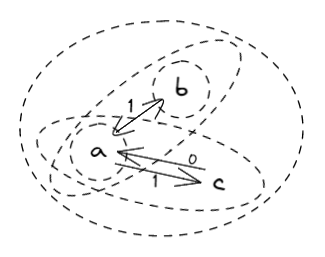
\includegraphics[width=0.35\textwidth]{Imagenes/grados_de_impacto.PNG}
  \caption{Grados de impacto para el espacio $X$ con la topología $\mathcal{A}$.}
  \label{fig:gradoImpacto}
\end{figure}

De la definición \ref{def:gradoDeImpacto} podemos deducir el siguiente resultado:

\newpage

\begin{teorema}\label{teo:gradeosDeImpactoImplicaSFV}
Los grados de impacto de una célula $x$ definen un sistema fundamental de vecindades.
\end{teorema}
\begin{proof}
Sea $x\in\mathcal{L}$ y $\mathcal{V}(x)$ una familia de vecindades de $x$. Defina el conjunto $A_0$ como el conjunto de puntos con grado de impacto con $x$ es igual a cero y de manera recursiva a los conjuntos $A_k$, cuyos elementos tienen grado de impacto con $x$ sea igual o menor a $k$. Claramente, $A_i\subseteq A_j$ para $0\leq i\leq j$ y de ese modo $A_i\in\mathcal{V}(x)$ para $i=0,1,\cdots,n$.

Veamos ahora que el conjunto $A_0$ es la vecindad mínimal de $x$. Considere $y\in U_x$, en particular $y\in\bigcap\mathcal{V}(x)$ por la definición de \ref{def:vecindadMinimal} Si el grado de impacto de $y$ con $x$ es mayor a cero por la definición \ref{def:gradoDeImpacto} podemos afirmar que existe $z\in\mathcal{L}$ tal que $z\thicksim x$, $z\thicksim y$ y $x\not\thicksim y$ y de ese modo $x$ e $y$ son puntos separables. Esto es una contradicción por el hecho de que $y\in \bigcap \mathcal{V}(x)$ y, por lo tanto $y\thicksim_0 x$, es decir $y\in A_0$.

Considere $y\in A_0$ y por la definición de grado de impacto cero, afirmamos que los puntos $x$ e $y$ no son separables por lo que $y\in V$ para todo $V\in\mathcal{V}(x)$ y de ese modo $y\in\bigcap\mathcal{V}(x)$, con lo que podemos concluimos la prueba.
\end{proof}

A continuación mostraremos algunas de las propiedades del conjunto $\mathcal{A}$ cuyos elementos son los conjuntos $A_k$ definidos en la demostración anterior.

\begin{proposicion}\label{pro:propiedadesSistemasDeVecindadesEncajadas}
Sea $x\in\mathcal{L}$ una célula y sea $\mathcal{A}$ la familia de conjuntos encajados definidos por el grado de impacto con $x$. Se cumplen las siguientes propiedades:
\begin{enumerate}
    \item El conjunto $\mathcal{A}$ posee elemento mínima igual a $A_0$,
    \item $\mathcal{A}$ es un conjunto ordenado finito con el orden de la contenencia, y
    \item $\mathcal{L}$ es un espacio uno-numerable.
\end{enumerate}
\end{proposicion}
\begin{proof}
Cada numeral se deduce directamente de las definiciones \ref{def:vecindadMinimal}, \ref{def:conjuntoPreordenadoFinito}, \ref{def:espacio1Numerable} y el teorema \ref{teo:gradeosDeImpactoImplicaSFV}.
\end{proof}

Algo que debemos tener en cuenta es que el grado de impacto por si solo no nos proporciona una medida del impacto que tienen los cambios de estado de células ``lejanas" (o de grado de impacto mayor a cero). Estas medidas de impacto se entenderán como la probabilidad de que un cambio de estado afecte a la célula con la que estamos realizando la comparación. De ese modo, las tasas de impacto serán valores entre 0 y 1 que pueden venir dados por cualquier tipo de función que tenga como dominio al conjunto de grados de impacto.

\begin{example}
Consideremos las siguientes matrices que describen los grados de impacto en tres distintos sistemas fundamentales de vecindades para la célula en la posición 2,2:

\begin{figure}[h]
  \centering
    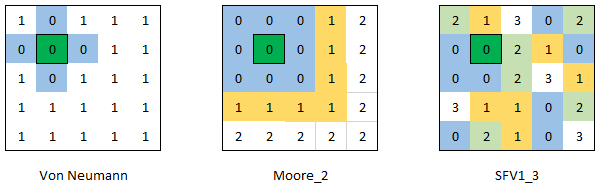
\includegraphics[width=0.75\textwidth]{Imagenes/ex315.PNG}
  \caption{Grados de impacto en diferentes sistemas de vecindades.}
  \label{fig:gradoImpacto}
\end{figure}

%%%%%%%%%%%%%%%%%%%%%%%%%%%%%%%%%%%%%%%%%%%%%%%%%%%%%%%%%%%%%%%%%%%%%%%%%%%%%%%%%%%%%%%%%%%%%
\newpage
%%%%%%%%%%%%%%%%%%%%%%%%%%%%%%%%%%%%%%%%%%%%%%%%%%%%%%%%%%%%%%%%%%%%%%%%%%%%%%%%%%%%%%%%%%%%%

Para implementar los grados de impacto descritos en la figura anterior tendremos que crear inicialmente un conjunto de células, como se muestra a continuación:

\begin{figure}[h]
  \centering
    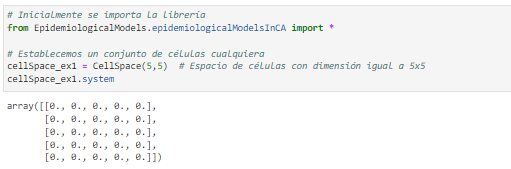
\includegraphics[width=1\textwidth]{Imagenes/interaccionesSociales1.png}
\end{figure}

Posteriormente, se definen manualmente los sistemas de vecindades junto con los grados de impacto de la siguiente manera

\begin{figure}[h]
  \centering
    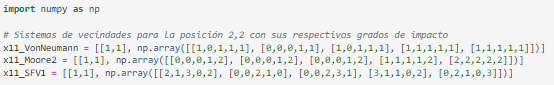
\includegraphics[width=1\textwidth]{Imagenes/interaccionesSociales2.png}
\end{figure}

En la figura (\ref{fig:gradoImpacto}) podemos ver que debido a la manera en la que implementamos nuestro espacio de células, es posible representar los grados de impacto de cada una con una célula particular en un arreglo matricial, al igual que los estados de cada célula, como se vio en el capítulo \ref{cap:Preliminares}.

La asignación entre grados y tasas de impacto puede escogerse de cualquier manera dependiendo del contexto y la enfermedad que esté modelando. Para los efectos del ejemplo, consideraremos las siguientes matrices de tasas de impacto (figura (\ref{fig:tasaImpacto})):

\begin{figure}[h]
  \centering
    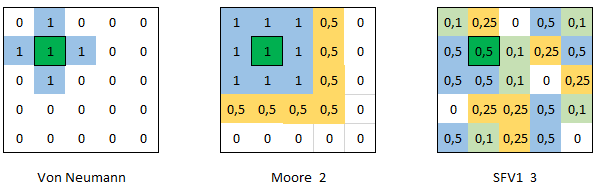
\includegraphics[width=0.75\textwidth]{Imagenes/ex3152.PNG}
  \caption{Tasas de impacto en diferentes sistemas de vecindades.}
  \label{fig:tasaImpacto}
\end{figure}
\end{example}

%%%%%%%%%%%%%%%%%%%%%%%%%%%%%%%%%%%%%%%%%%%%%%%%%%%%%%%%%%%%%%%%%%%%%%%%%%%%%%%%%%%%%%%%%%%%%
\newpage
%%%%%%%%%%%%%%%%%%%%%%%%%%%%%%%%%%%%%%%%%%%%%%%%%%%%%%%%%%%%%%%%%%%%%%%%%%%%%%%%%%%%%%%%%%%%%

Para establecer las tasas de impacto basta con agregarlas de manera ordenada a una lista, como se muestra en el siguiente script:

\begin{figure}[h]
  \centering
    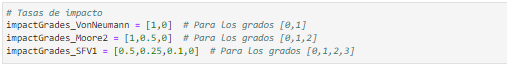
\includegraphics[width=1\textwidth]{Imagenes/interaccionesSociales3.png}
\end{figure}

Una vez establecidos los conceptos de topología implementados para nuestro espacio $\mathcal{L}$ y sus sistemas fundamentales de vecindades podemos definir cada una de las reglas que implementaremos para cada modelo epidemiológico.

\section{Reglas de evolución}\label{sec:ReglasDeEvolución}

Partiremos de una abstracción sobre la naturaleza de los modelos epidemiológicos definidos en el capítulo \ref{cap:Preliminares}, esto nos permitirá definir de manera intuitiva las reglas de evolución de nuestros modelos en autómatas celulares.

Antes de comenzar a definir nuestras reglas de evolución definiremos las siguientes notaciones:
\begin{itemize}
    \item El estado de la célula $x$ en un momento $t$ se denotará como $\pi^t(x)$.
    \item La cantidad de individuos con grado de impacto $g$ y estado $K$ de una célula $x$ en un momento $t$, será representado como $\sigma_{g,K}^t(x)$.
    \item Para representar a la cantidad de individuos con un grado de impacto $g$ usaremos el símbolo $\Delta_g$. 
    \item Usaremos los símbolos $\mathcal{S}^t,\mathcal{I}^t,\mathcal{R}^t$ y $\mathcal{D}^t$ para denotar a los conjuntos de células susceptibles, infectadas, recuperadas y muertas respectivamente en el espacio $\mathcal{L}$ en el tiempo $t$. De manera formal
    $$\mathcal{S}^t=\{x\in\mathcal{L}:\pi^t(x)=S\},$$
    y de manera análoga se definen los conjuntos $\mathcal{I}^t,\mathcal{R}^t$ y $\mathcal{D}^t$. Note que $$\mathcal{S}^t\cup\mathcal{I}^t\cup\mathcal{R}^t\cup\mathcal{D}^t=\mathcal{L}\text{ para todo tiempo }t.$$
\end{itemize}

\subsection{Modelos SIS y SIR simples}\label{sub:SISySIRSimples}

Recordemos que para las tasas de infección $\beta$ y de recuperación $\alpha$, los modelos SIS y SIR en su versión más simple, nos afirman que para $\mathcal{R}_0=\frac{\beta}{\alpha}>1$ la enfermedad será endémica. Trataremos de replicar inicialmente esté comportamiento de manera local sobre una célula analizando los siguientes puntos:

\begin{itemize}
    \item La probabilidad de que un individuo susceptible se enferme depende no solo de la enfermedad, sino que también se debe considerar a la cantidad de individuos infectados que tenga en su sistema de vecindades locales, atada a las tasas de impacto que definimos en la sección anterior. 
    \item Como vimos en el capítulo \ref{cap:Preliminares}, la recuperación de los individuos infectados no se ve afectada por la cantidad de contactos con otras células y en lugar de eso, depende completamente de la tasa de recuperación $\alpha$, la cual en nuestro caso entenderemos como la proporción de individuos infectados que se recuperan de la enfermedad.
    \item Para el estado de inmunidad en el modelo SIR, supondremos que los individuos que posean este estado se mantendrán inmunes. Esto quiere decir que la transformación para individuos recuperados será constante e igual a $R$ (recuperado).
\end{itemize}

Dado que los modelos SIS y SIR comparten el paso del estado S al estado I definiremos primero la regla de evolución para un modelo SI como sigue:

\begin{definition}\label{def:reglaSI}
Para una célula $x$ en un espacio $\mathcal{L}$ definimos la regla SI como:
\begin{equation}
    \phi_{SI}^t(x)=\left\{\begin{array}{ll}
        S & \text{si }\pi^t(x)=S\text{, }\sum_g{\sigma_{g,I}^t(x)\cdot P(g)}\leq \sum_g{\sigma_{g,S}^t(x)\cdot P(g)}\text{ y }\rho\geq i(t),\\
        I & \text{si }\pi^t(x)\in\{S,I\}\text{,} \\
        \pi^t(x) & \text{en otro caso,}
    \end{array}\right.
\end{equation}
con $\rho\in\mathcal{U}_{[0,1]}$, $P(g)$ la tasa de impacto del grado $g$ e
\begin{equation}
    i(t) = \frac{\beta}{\alpha}\sum_g{\frac{\sigma_{g,I}^t(x)}{\Delta_g}}\cdot P(g),
\end{equation}
donde el factor $\frac{\beta}{\alpha}$ indica la afectación ocasionada por la enfermedad y el factor restante corresponde al comportamiento de las células y su impacto en la célula $x$.
\end{definition}

\newpage

\begin{definition}\label{def:nivelIncidencia}
Las sumatorias $\sum_g{\sigma_{g,S}^t(x)\cdot P(g)}$ y $\sum_g{\sigma_{g,I}^t(x)\cdot P(g)}$ de la definición anterior, serán conocidas como el nivel de incidencia de las células con estados $S$ e $I$ sobre una célula $x$ respectivamente.
\end{definition}

\textit{Observación:} La definición \ref{def:nivelIncidencia} se puede extender a un estado $\sigma$ cualquiera tomando a la sumatoria $\sum_g{\sigma_{g,\sigma}^t(x)\cdot P(g)}$ para una célula $x$ y un conjunto de grados de impacto establecidos previamente.

\begin{example}\label{ex:SIenAutómatasCelulares}
En la figura (\ref{fig:configuraciónInicialEspacio25Celulas}) podemos encontrar la configuración de estados para un sistema de 25 células: en las tres del lado derecho encontramos la disposición de grados de impacto para las tres células marcadas en color naranja (primera imagen), donde SFV es una abreviación de Sistema Fundamental de Vecindades.

%%%%%%%%%%%%%%%%%%%%%%%%%%%%%%%%%%%%%%%%%%%%%%%%%%%%%%%%%%%%%%%%%%%%%%%%%%%%%%%%%%%%%%%%%%%%%%%%%
%\newpage
%%%%%%%%%%%%%%%%%%%%%%%%%%%%%%%%%%%%%%%%%%%%%%%%%%%%%%%%%%%%%%%%%%%%%%%%%%%%%%%%%%%%%%%%%%%%%%%%%

\begin{figure}[h]
  \centering
    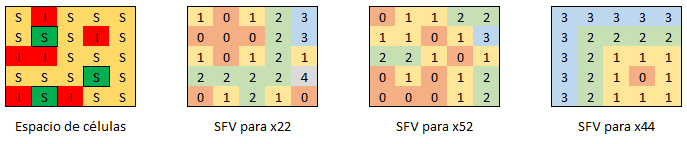
\includegraphics[width=0.95\textwidth]{Imagenes/cellSpace.PNG}
    \caption{Configuración inicial de estados y sistemas fundamentales de vecindades}
    \label{fig:configuraciónInicialEspacio25Celulas}
\end{figure}

Consideraremos las siguientes tasas de impacto:

\begin{table}[h]
\begin{center}
\begin{tabular}{| c | c |}
\hline
Grados & Tasas \\ \hline
0 & 0.5 \\
1 & 0.3\\
2 & 0.25\\
3 & 0.1\\ 
4 & 0.05\\ \hline
\end{tabular}
\caption{Relación entre tasas y grados de impacto.}
\end{center}
\end{table}

A continuación calcularemos las magnitudes ponderadas de individuos susceptibles e infectados y la probabilidad de infectarse para cada una de las tres células:

\begin{itemize}
    \item Célula $x_{2,2}$:
    \begin{align*}
    \begin{array}{l}
        \sum_g\sigma_{g,S}^0(x_{2,2})\cdot P(g) = 4\cdot0.5+6\cdot0.3+6\cdot0.25+2\cdot0.1+1\cdot0.05 = 5.55 \\
        \sum_g\sigma_{g,I}^0(x_{2,2})\cdot P(g) = 3\cdot0.5+1\cdot0.3+2\cdot0.25+0\cdot0.1+0\cdot0.05 = 2.3\\
        i_{2,2}(0) = \frac{\beta}{\alpha}\cdot\left(\frac{3\cdot0.5}{7}+\frac{1\cdot0.3}{7}+\frac{2\cdot0.25}{8}+\frac{0\cdot0.1}{2}+\frac{0\cdot0.05}{1}\right)=\frac{\beta}{\alpha}\cdot\frac{179}{560}
    \end{array}
    \end{align*}
    \item Célula $x_{5,2}$:
    \begin{align*}
    \begin{array}{l}
        \sum_g\sigma_{g,S}^0(x_{5,2})\cdot P(g) = 6\cdot0.5+8\cdot0.3+4\cdot0.25+1\cdot0.1+0\cdot0.05 = 6.5 \\
        \sum_g\sigma_{g,I}^0(x_{5,2})\cdot P(g) = 2\cdot0.5+2\cdot0.3+2\cdot0.25+0\cdot0.1+0\cdot0.05 = 2.1\\
        i_{5,2}(0) = \frac{\beta}{\alpha}\cdot\left(\frac{2\cdot0.5}{8}+\frac{2\cdot0.3}{10}+\frac{2\cdot0.25}{6}+\frac{0\cdot0.1}{1}\right)=\frac{\beta}{\alpha}\cdot\frac{161}{600}
    \end{array}
    \end{align*}
    \item Célula $x_{4,4}$:
    \begin{align*}
    \begin{array}{l}
        \sum_g\sigma_{g,S}^0(x_{4,4})\cdot P(g) = 1\cdot0.5+7\cdot0.3+5\cdot0.25+6\cdot0.1+0\cdot0.05 = 4.45 \\
        \sum_g\sigma_{g,I}^0(x_{4,4})\cdot P(g) = 0\cdot0.5+1\cdot0.3+2\cdot0.25+3\cdot0.1+0\cdot0.05 = 1.1\\
        i_{4,4}(0) = \frac{\beta}{\alpha}\cdot\left(\frac{0\cdot0.5}{1}+\frac{1\cdot0.3}{8}+\frac{2\cdot0.25}{7}+\frac{3\cdot0.1}{9}\right)=\frac{\beta}{\alpha}\cdot\frac{239}{1680}
    \end{array}
    \end{align*}
\end{itemize}

Podemos apreciar que los niveles de incidencia para los estados del modelo son diferentes para cada una de las células que consideramos. Esto implica que las probabilidades de contagiarse de la enfermedad están directamente relacionados con la manera en la que las células interactúan entre sí.

En este caso las tres células pueden o no contagiarse de la enfermedad si aplicamos la regla $\phi_{SI}^t(x)$. Supongamos que la enfermedad cuenta con una tasa de infección $\beta=0.5$ y una tasa $\alpha=0.2$, de ese modo las probabilidades de adquirir la enfermedad son:
$$\begin{array}{ccccc}
    i_{2,2}(0)=0.8, & i_{5,2}(0)=0.675. & \text{e} & i_{4,4}(0)=0.35.
\end{array}$$
Podemos observar que la célula $x_{4,4}$ tiene una probabilidad menor de adquirir la enfermedad y esto se debe a que según el sistema de vecindades escogido, la célula se encuentra más alejada de los infectados que las células $x_{2,2}$ y $x_{5,2}$.
\end{example}

\textit{Nota:} Puede consultar la implementación de la definición \ref{def:reglaSI} en el módulo \href{https://github.com/Grupo-de-simulacion-con-automatas/Prediccion-del-comportamiento-de-una-enfermedad-simulada-en-AC-con-un-algoritmo-en-RN/blob/master/Codigo/CAsimulation/casimulation/Models.py#:~:text=def-,__SI_rule,-(self\%2C\%20cellState\%2C\%20neighborsByImpact}{\underline{Models}} de la librería. \\

La definición \ref{def:reglaSI} nos permite definir de manera natural a las reglas de evolución para los modelos SIS y SIR en autómatas celulares:

\begin{definition}\label{def:reglasSISySIR}
Dada una célula $x$ en un conjunto $\mathcal{L}$ definimos respectivamente las reglas de evolución para los modelos SIS y SIR respectivamente como:
\begin{equation}
    \phi_{SIS}^t(x)=\left\{\begin{array}{ll}
        \phi_{SI}^t(x) & \text{si }\pi^t(x) = S,\\
        I & \text{si }\pi^t(x)=I\text{ y }\rho>\alpha,\\
        S & \text{si }\pi^t(x)=I\text{ y }\rho\leq\alpha.
    \end{array}\right.
\end{equation}

\begin{equation}
    \phi_{SIR}^t(x)=\left\{\begin{array}{ll}
        \phi_{SI}^t(x) & \text{si }\pi^t(x) = S,\\
        I & \text{si }\pi^t(x)=I\text{ y }\rho>\alpha,\\
        R & \text{si }\pi^t(x)=I\text{ y }\rho\leq\alpha, y \\
        R & \text{si }\pi^t(x)=R,
    \end{array}\right.
\end{equation}
donde $\rho\in\mathcal{U}_{[0,1]}$.
\end{definition}

\textit{Observación:} Dado que las reglas $\phi_{SIS}^t(x)$ y $\phi_{SIR}^t(x)$ actúan como una composición de funciones para el estado $I$, debemos conocer primero a los individuos que se recuperan de la enfermedad, esto significa que computacionalmente tendremos que aplicar primero la regla $\phi_{IR}^t(x)$ (o $\phi_{IS}^t(x)$ en el caso del modelo SIS) y luego las probabilidades de infección sobre los individuos susceptibles.



\begin{example}\label{ex:SISySIRenAutomatasCelulares}
Consideremos la configuración de estados del ejemplo anterior junto con las tasas de infección y recuperación $\beta=0.5$ y $\alpha=0.2$ respectivamente. De acuerdo con la definición \ref{def:reglaSI} y la observación anterior, si aplicamos las reglas $\phi_{SIS}^t(x)$ y $\phi_{SIR}^t(x)$ podremos observar un comportamiento similar a los siguientes:

%%%%%%%%%%%%%%%%%%%%%%%%%%%%%%%%%%%%%%%%%%%%%%%%%%%%%%%%%%%%%%%%%%%%%%%%%%%%%%%%%%%%%%%%%%%%%%%%%
% \newpage
%%%%%%%%%%%%%%%%%%%%%%%%%%%%%%%%%%%%%%%%%%%%%%%%%%%%%%%%%%%%%%%%%%%%%%%%%%%%%%%%%%%%%%%%%%%%%%%%%

\begin{figure}[h]
  \centering
    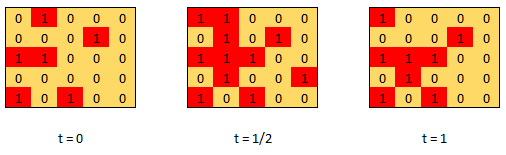
\includegraphics[width=0.7\textwidth]{Imagenes/sisAplication.PNG}
    \caption{Aplicación de la regla $\phi_{SIS}^t(x)$}
\end{figure}
\vspace{-0.5cm}
\begin{figure}[h]
  \centering
    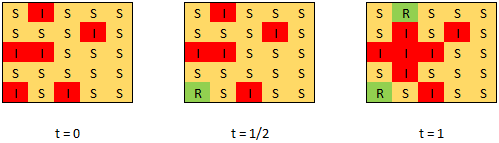
\includegraphics[width=0.7\textwidth]{Imagenes/sirAplication.PNG}
    \caption{Aplicación de la regla $\phi_{SIR}^t(x)$}
\end{figure}

Como se puede observar en la aplicación de ambas reglas, existe una unidad temporal intermedia en la que se aplica la regla sobre el estado $I$ para luego aplicar la regla $\phi_{SI}^t(x)$. En el caso del modelo SIS vemos que las células pasan al estado $S$ de acuerdo con las reglas del modelo clásico y de manera similar con el modelo SIR.
\end{example}

\textit{Observación:} Es importante recordar que el paso del estado $I$ al estado $S$ (o al $R$) no depende del sistema de vecindades, ya que se asume que no es necesario el contacto con células no infectadas para que una que se encuentra enferma se recupere.

\begin{example}\label{ex:SISySIRclásicovsModeloEnAC}
Consideremos dos espacios de 900 células en donde una misma enfermedad actúa de manera diferente en el sentido de que mientras en el primer espacio los individuos no generan inmunidad tras recuperarse de la enfermedad, en el segundo espacio si y durante un tiempo indefinido.

Las tasas de infección y de recuperación de la enfermedad son $\beta=0.5$ y $\alpha=0.2$, lo que implica que la enfermedad será endémica, pues $\mathcal{R}_0=\frac{\beta}{\alpha}=2.5>1$. Asumiremos que el brote de infectados inicial se ubicó en la zona central de ambos espacios y que las interacciones entre células se describen a partir del sistema de vecindades generado por las vecindades de Moore. La evolución de la enfermedad en ambos espacios se puede apreciar en las figuras (\ref{fig:sisEn30}) y (\ref{fig:sirEn30}).

Definimos los parámetros tanto del espacio de células como de la enfermedad:

\begin{figure}[h]
  \centering
    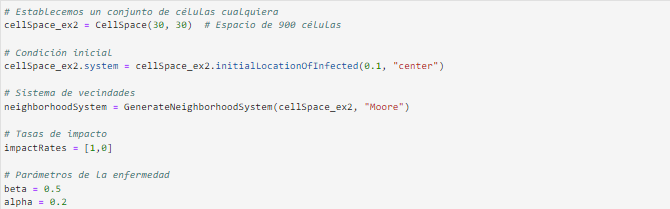
\includegraphics[width=1\textwidth]{Imagenes/interaccionesSociales4.png}
\end{figure}

Una vez definidos los parámetros procedemos a aplicar las reglas de evolución de ambos modelos. Como se puede apreciar en los siguientes fragmentos, se ofrece la posibilidad de visualizar los comportamientos espaciales luego de haber aplicado los modelos:

\begin{figure}[h]
  \centering
    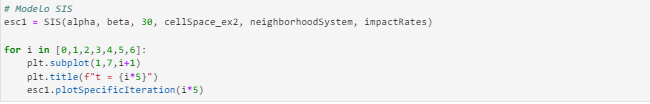
\includegraphics[width=1\textwidth]{Imagenes/interaccionesSociales5.png}
\end{figure}
\vspace{-0.5cm}
\begin{figure}[h]
  \centering
    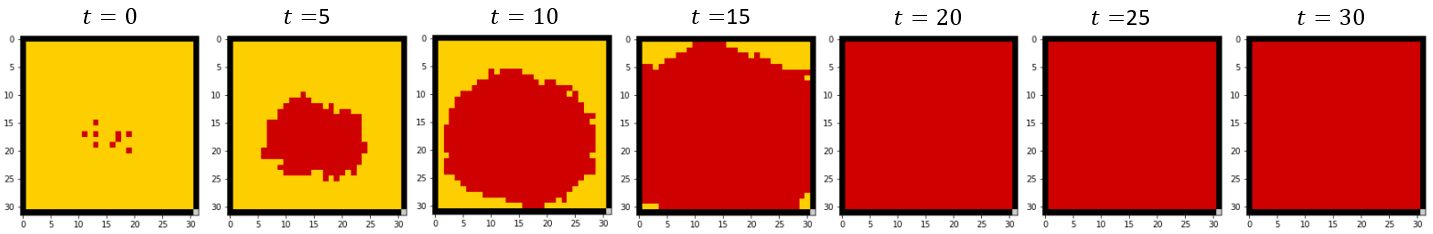
\includegraphics[width=1\textwidth]{Imagenes/sisEn30.PNG}
    \caption{Evolución de la enfermedad en 30 días (modelo SIS).}
    \label{fig:sisEn30}
\end{figure}
\vspace{-0.5cm}
\begin{figure}[h]
  \centering
    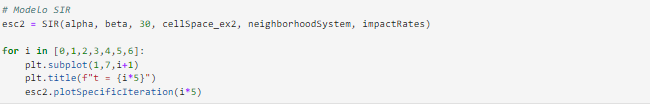
\includegraphics[width=1\textwidth]{Imagenes/interaccionesSociales6.png}
\end{figure}
\vspace{-0.5cm}
\newpage

\begin{figure}[h]
  \centering
    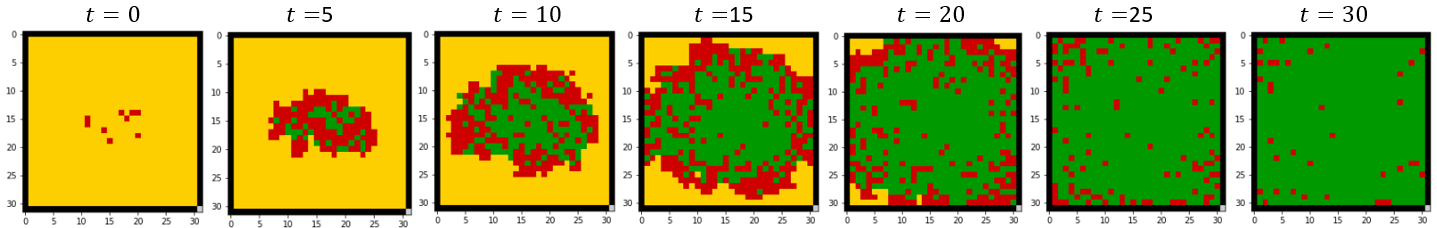
\includegraphics[width=1\textwidth]{Imagenes/sirEn30.PNG}
    \caption{Evolución de la enfermedad en 30 días (modelo SIR).}
    \label{fig:sirEn30}
\end{figure}
En la figura (\ref{fig:comparacionReglasvsClasico}) podremos visualizar las soluciones obtenidas al analizar el mismo escenario con los modelos clásicos (izquierda) y las generadas por nuestras reglas de evolución $\phi_{SIS}^t(x)$ y $\phi_{SIR}^t(x)$ (derecha). Para generar las gráficas del lado derecho (reglas SIS y SIR definidas durante esta sección) utilizaremos el siguiente script:

\begin{figure}[h]
  \centering
    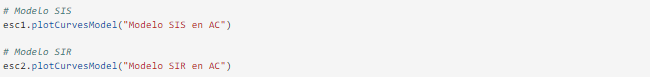
\includegraphics[width=1\textwidth]{Imagenes/interaccionesSociales7.png}
    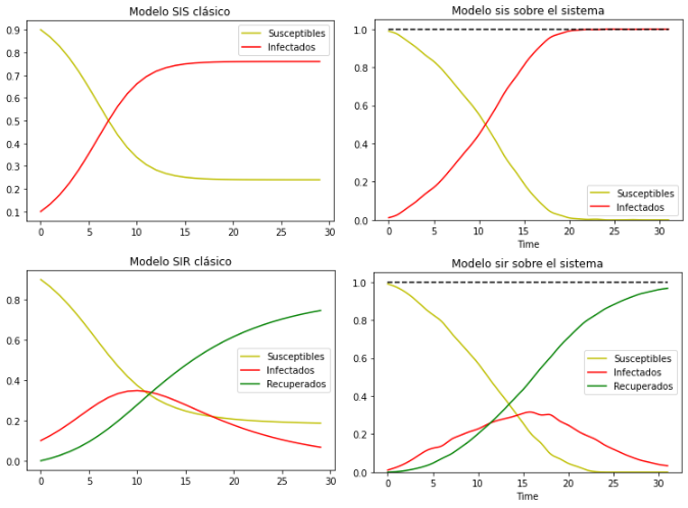
\includegraphics[width=0.55\textwidth]{Imagenes/solucionesSISySIR1.PNG}
    \caption{Evolución de la enfermedad en 30 días (modelos clásicos vs reglas de evolución).}
    \label{fig:comparacionReglasvsClasico}
\end{figure}
\end{example}
\textit{Nota:} Al igual que para la regla SI, brindamos al lector la posibilidad de consultar las reglas \href{https://github.com/Grupo-de-simulacion-con-automatas/Prediccion-del-comportamiento-de-una-enfermedad-simulada-en-AC-con-un-algoritmo-en-RN/blob/master/Codigo/EpidemiologicalModels/Models.py#:~:text=class-,SISmodel,-(SImodel)\%3A}{\underline{SIS}} y \href{https://github.com/Grupo-de-simulacion-con-automatas/Prediccion-del-comportamiento-de-una-enfermedad-simulada-en-AC-con-un-algoritmo-en-RN/blob/master/Codigo/EpidemiologicalModels/Models.py#:~:text=class-,SIRmodel,-(SImodel)\%3A}{\underline{SIR}} en el módulo Models de la librería CAsimulations.

\subsection{Modelos con natalidad y mortalidad}\label{sub:NatalidadyMortalidad}
Partiendo del principio de que los análisis desarrollados en nuestra investigación tengan una mayor aplicabilidad en el ámbito epidemiológico, decidimos separarnos un poco de los modelos clásicos, ya que en estos se supone que las tasas de natalidad y mortalidad son iguales y esto no necesariamente se cumple en el mundo real.

La segunda característica que tendremos en mente para definir nuestra regla de evolución parte de la hipótesis de que los individuos en un sistema tienen una probabilidad de fallecer por causas ajenas a la enfermedad que depende de la edad del mismo individuo.

Para implementar la noción de edad de una célula inicialmente tendremos que modificar el dominio de nuestra regla de evolución. Para estos modelos debemos tener en cuenta el estado de la célula central junto con su edad y el estado de sus vecinos, de modo que 
$$Dom(\phi_\mu)=\Sigma_x\times K\times\overbrace{\Sigma\times\cdots\times\Sigma}^N\text{, con }K=\{1,2,\cdots,100\},$$
si suponemos que la edad de la célula $x$ puede ir de 1 a 100 unidades temporales (semanas, meses, años, etc.).

Otra característica que podemos implementar en nuestro modelo es la del envejecimiento de las células, esto con el objetivo de analizar el impacto de una enfermedad sobre los individuos de un sistema en diferentes etapas de su ``vida". La manera en la que abordaremos esta idea será con el siguiente ajuste en el rango de nuestra regla
$$Ran(\phi_\mu)=\Sigma_x\times K.$$
Dado que estamos trabajando sobre poblaciones de tamaño constante la manera en la que interpretaremos el nacimiento de una célula será con la ocupación del espacio que deja una que muere. Para esto identificaremos a los espacios que dejan las células que mueren con el estado $D$ y una edad cero, esto nos permitirá separar a los espacios que pueden ocuparse y los que no de células que interactúen con sus vecinos. Al igual que en los modelos descritos en el capítulo \ref{cap:Preliminares}, asumiremos que los individuos que ``nacen" son susceptibles a la enfermedad.

Teniendo estas ideas en mente podemos definir la regla de evolución para un modelo epidemiológico $M$ de la siguiente manera:

\begin{definition}\label{def:reglaNatalidadyMortalidad}
Sea $x$ una célula en un conjunto $\mathcal{L}$, $M$ un modelo epidemiológico ($SIS, SIR$, etc.) y $T$ una unidad temporal (días, meses, años, etc.). Definimos la regla de evolución con nacimientos y muertes para $M$ como:
\begin{equation}
    \mu_{M,T}^t(x)=\left\{\begin{array}{ll}
        D,0 & \text{si }t\not\equiv 0 \text{ (modulo }T\text{), }\pi^t(x)\in\{S,I,R\}\text{ y }\rho\leq\omega_k, \\
        D,0 & \text{si }\pi^t(x)=D\text{ y }\rho>b,\\
        S,1 & \text{si }\pi^t(x)=D\text{ y }\rho\leq b,\\
        \phi_M^t(x),E^t(x) & \text{si }t\not\equiv 0 \text{ (modulo }T),\\
        \phi_M^t(x),E^t(x)+1 & \text{si }t\equiv 0 \text{ (modulo }T),
    \end{array}\right.
\end{equation}
donde $\omega_k$ es la probabilidad de morir por causas ajenas a la enfermedad para las edades en la partición k-ésima del intervalo $[0,100]$, $b$ es la tasa de natalidad, $\phi_M^t$ es la regla de evolución del modelo epidemiológico, $E^t(x)$ denota la edad de la célula $x$ en el momento $t$ y $\rho\in\mathcal{U}_{[0,1]}$.
\end{definition}

\textit{Observación:} La distribución de probabilidad con la que se escoge a $\rho$ puede no ser uniforme y en su lugar depender del fenómeno que se esté modelando. Para los objetivos del proyecto nos enfocaremos únicamente en la distribución uniforme y esperamos profundizar en futuras investigaciones en analizar el nivel de afectación que puede tener la escogencia de diferentes distribuciones de probabilidad.

\begin{example}\label{ex:natalidadyMortalidad}
Consideremos una probabilidad de nacimiento (u ocupación de espacios disponibles) $b=0.02$ y una unidad temporal $T=2$ sobre la siguiente configuración de estados en un espacio de células junto con las probabilidades de muerte por grupo de edad: 

\begin{figure}[h]
  \centering
    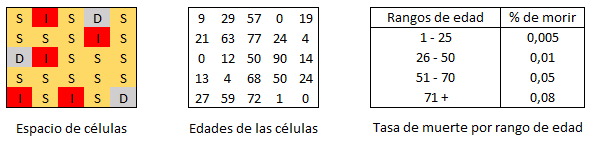
\includegraphics[width=0.8\textwidth]{Imagenes/conInicialMNM.PNG}
    \caption{Configuración inicial para el espacio de células y tasas de muerte por edad.}
    \label{ex:configuraciónInicialNatalidadyMortalidad}
\end{figure}

Dado que las células que posean una edad igual a cero no podrán interactuar con las demás debido a su misma definición, podemos afirmar que existe una dependencia entre el estado de la célula y su edad por lo que antes de aplicar la regla de evolución del modelo epidemiológico (SIS o SIR), aplicaremos la regla para los cambios sobre las edades de la célula de acuerdo con la definición \ref{def:reglaNatalidadyMortalidad}.

\begin{figure}[h]
  \centering
    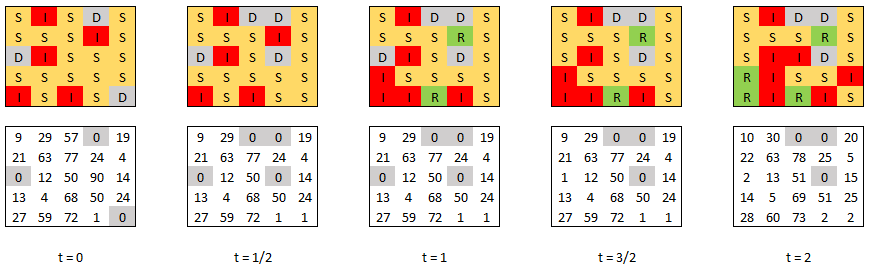
\includegraphics[width=1\textwidth]{Imagenes/natalidadMortalidad.PNG}
    \caption{Aplicación de la regla $\mu_{SIR,2}^t(x)$}
    \label{ex:aplicaciónReglaNatalidadyMortalidad}
\end{figure}

En la figura (\ref{ex:aplicaciónReglaNatalidadyMortalidad}) podemos observar la aplicación del modelo SIR con natalidad y mortalidad en donde en particular en los tiempos $t=1/2$ y $t=3/2$ mueren y nacen nuevas células de acuerdo con las probabilidades de muerte por rango de edad y tasa de nacimiento establecidas. Por otra parte y de acuerdo con la definición del parámetro $T$, todas las células cumplen un ciclo (que puede entenderse como un año) cuando $t\equiv0$ (Módulo $T$).
\end{example}

\begin{example}\label{ex:sisClásicovsModeloEnAC}
Consideremos ahora una enfermedad que actúa sobre un espacio de 100 células y que posee tasas de infección y de recuperación, $\beta=0.05$ y $\alpha=0.2$ respectivamente. Para comparar los resultados con el modelo clásico asumiremos que las tasas de natalidad y mortalidad son iguales a $\mu=\frac{1}{75\cdot6}$ (esperanza de vida de 75 años y $T=6$, es decir, las medidas se toman cada 2 meses). En particular podemos observar que la enfermedad no será endémica, pues $\mathcal{R}_0=\frac{\beta}{\alpha+\mu}\approx0.25<1$.

Inicialmente, definimos tanto los parámetros espaciales como los parámetros de la enfermedad, de la siguiente manera:

\begin{figure}[h]
  \centering
    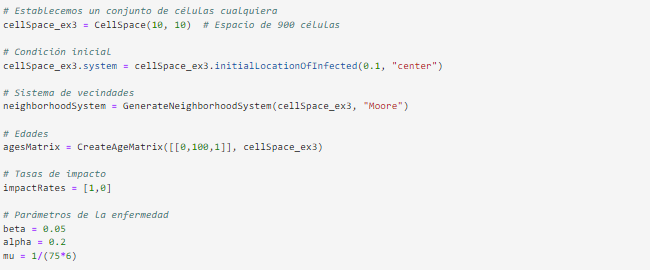
\includegraphics[width=1\textwidth]{Imagenes/interaccionesSociales8.png}
\end{figure}
\begin{figure}[h]
  \centering
    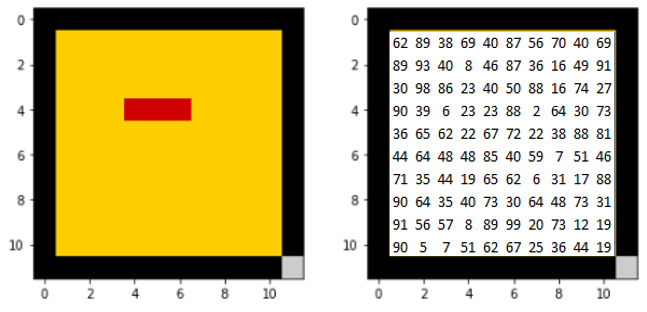
\includegraphics[width=0.6\textwidth]{Imagenes/sistemaYEdades.PNG}
    \caption{Configuración inicial de estados y de edades}
    \label{ex:aplicaciónReglaNatalidadyMortalidad}
\end{figure}

A continuación ejecutaremos 30 veces la regla de evolución $\mu_{SIS,6}^t(x)$ y comparemos los resultados con los generados por el modelo clásico (figura (\ref{ex:aplicaciónReglaNatalidadyMortalidad})). Podemos observar que en ambos casos la población de infectados tiende a cero y que la cantidad de espacios libres (o células muertas) no crece demasiado, esto se debe a la baja probabilidad de muerte de nuestro espacio de células.

\begin{figure}[h]
  \centering
    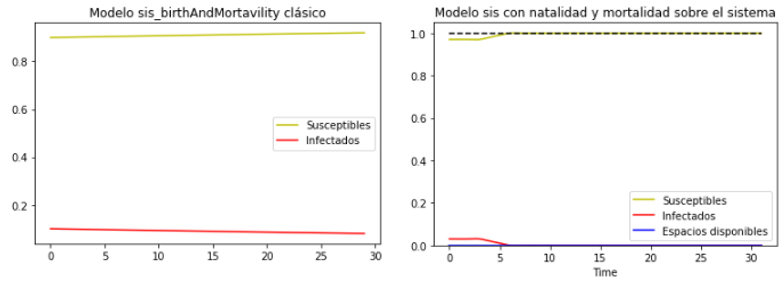
\includegraphics[width=0.75\textwidth]{Imagenes/solucionesNatalidadYMortalidad.PNG}
    \caption{Evolución de la enfermedad en 30 bimestres (modelo clásico y regla $\mu_{SIS,6}^t(x)$)}
    \label{ex:aplicaciónReglaNatalidadyMortalidad}
\end{figure}

Para generar una gráfica como la de la derecha puede ejecutar el siguiente script una vez tenga definidos los parámetros del modelo:
\begin{figure}[h]
  \centering
    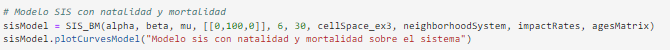
\includegraphics[width=1\textwidth]{Imagenes/interaccionesSociales9.png}
\end{figure}
\end{example}

\textit{Nota:} Al igual que para las reglas anteriores, se brinda al lector la posibilidad de consultar la regla para los  \href{https://github.com/Grupo-de-simulacion-con-automatas/CAsimulations-Modelacion-de-dinamicas-topologicas-en-la-propagacion-de-una-enfermedad-usando-CA/blob/master/Codigo/CAsimulation/casimulation/Models.py#:~:text=class-,birthAndMortavility,-\%3A}{\underline{modelos con natalidad y mortalidad}} en el módulo Models de la librería CAsimulations.

\subsection{Modelos con muerte por enfermedad}\label{sub:MuertePorEnfermedad}
En esta sección nos enfocaremos en definir la versión más general de los modelos epidemiológicos clásicos en ecuaciones diferenciales definidas en el capítulo \ref{cap:Preliminares}. La muerte por enfermedad afectará únicamente a las células que posean la enfermedad y, buscando una mayor aplicabilidad sobre eventos más realistas asumiremos que la enfermedad puede tener distintos grados de mortalidad para rangos de edad diferentes. 

Al igual que en la sección anterior, realizaremos una partición sobre el intervalo $[0,100]$ y definiremos una probabilidad $\theta_k$ que indique la probabilidad de morir a causa de la enfermedad en la k-ésima partición. Teniendo esto en mente, podemos definir a la regla de evolución para modelos epidemiológicos con muerte por enfermedad como sigue:

\begin{definition}\label{def:reglaMuertePorEnfermedad}
Sea $x$ una célula en un conjunto $\mathcal{L}$, $M$ un modelo epidemiológico ($SIS$, $SIR$, etc.) y $T$ una unidad temporal (días, meses, años, etc.). Definimos la regla de evolución con muerte por enfermedad para $M$ como:
\begin{equation}
    \theta_{M,T}^t(x)=\left\{\begin{array}{ll}
        D,0 & \text{si }\pi^t(x)=I\text{ y }\rho\leq\theta_k, \\
        \mu_{M,T}^t(x) & \text{en otro caso.}
    \end{array}\right.
\end{equation}
Donde $\theta_k$ es la probabilidad de morir por la enfermedad para los individuos con una edad en el intervalo k-ésimo de la partición del intervalo $[0,100]$, $\mu_{M,T}^t$ es la regla de evolución para modelos con nacimientos y muertes y $\rho\in\mathcal{U}_{[0,1]}$.
\end{definition}

\begin{example}
Partiremos del mismo escenario considerado en el ejemplo \ref{ex:natalidadyMortalidad} con las siguientes probabilidades de muerte por grupo de edad:

\begin{figure}[h]
  \centering
    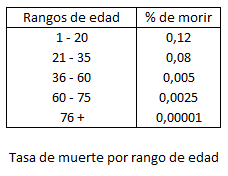
\includegraphics[width=0.3\textwidth]{Imagenes/muertePorEnfermedad.PNG}
\end{figure}

Al igual que en el ejemplo \ref{ex:natalidadyMortalidad}, la aplicación de la regla de evolución se realizará en dos fases: la primera fase corresponderá a los nacimientos, muertes por causas naturales, cambios en las edades de las células y la aplicación de las tasas de muerte causada por enfermedad por grupo de edad sobre los infectados y seguido de esto, se aplicará el modelo epidemiológico que corresponde a la segunda fase de nuestra regla de evolución.

\begin{figure}[h]
  \centering
    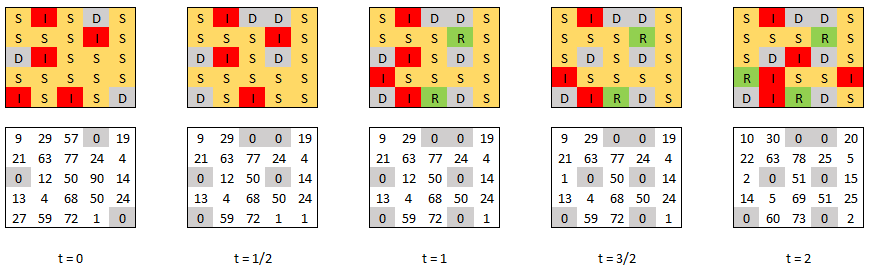
\includegraphics[width=1\textwidth]{Imagenes/muertePorEnfermedadEvo.PNG}
    \caption{Aplicación de la regla $\theta_{SIR,2}^t(x)$}
\end{figure}
\end{example}

\textit{Nota:} Al igual que para las reglas anteriores, se brinda al lector la posibilidad de consultar la regla para los  \href{https://github.com/Grupo-de-simulacion-con-automatas/CAsimulations-Modelacion-de-dinamicas-topologicas-en-la-propagacion-de-una-enfermedad-usando-CA/blob/master/Codigo/CAsimulation/casimulation/Models.py#:~:text=class-,deathByDisease,-\%3A}{\underline{modelos con muerte por enfermedad}} en el módulo Models de la librería CAsimulations.

\begin{example}\label{ex:muertePorEnfermedadClásicovsModeloEnAC}
Partiremos de la misma configuración de edades sobre un sistema de 100 células y las mismas tasas de natalidad y mortalidad consideradas en el ejemplo \ref{ex:aplicaciónReglaNatalidadyMortalidad}. Tomaremos las vecindades de Von Neumann para describir sus interacciones. En cuanto a la enfermedad, supondremos una tasa de infección $\beta=0.5$, una de recuperación $\alpha=0.2$ y una probabilidad de muerte causada por la misma enfermedad de $\theta=0.4$ (tomamos este valor con el objetivo de comparar los resultados con el modelo clásico).

\begin{figure}[h]
  \centering
    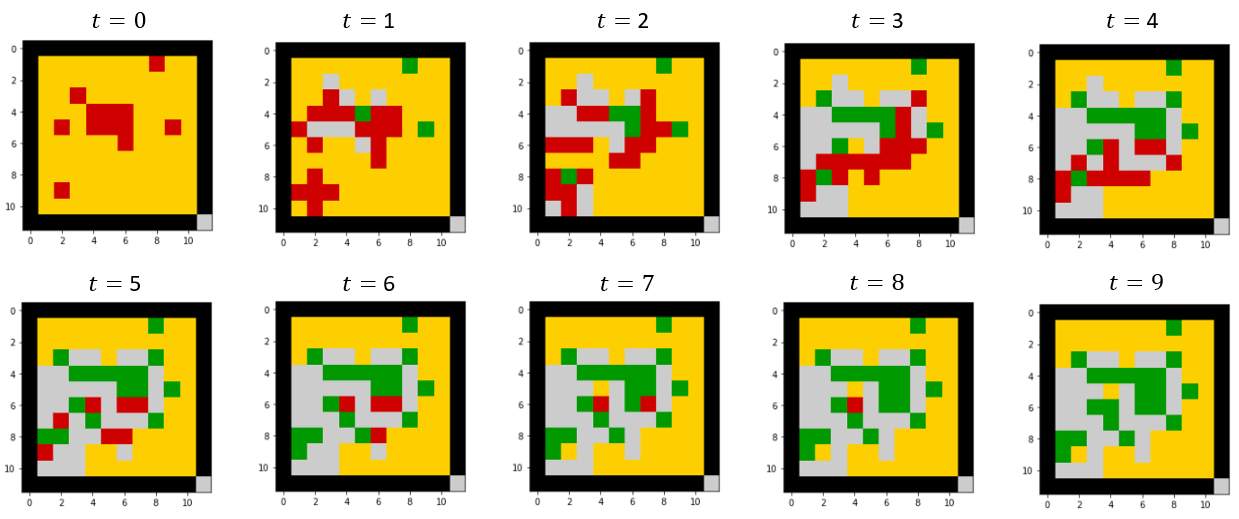
\includegraphics[width=1\textwidth]{Imagenes/evolucionesMuertePorEnfermedad.PNG}
    \caption{Aplicación de la regla $\theta_{SIR,6}^t(x)$ en 10 iteraciones}
    \label{fig:muertePorEnfermedad10Veces}
\end{figure}

En la figura (\ref{fig:muertePorEnfermedad10Veces}) podemos observar que hay un incremento bastante pronunciado desde la segunda iteración hasta la quinta debido a la alta mortalidad de la enfermedad.

Una de las ventajas que ofrece nuestra librería es la de aplicar la regla de evolución varias veces y visualizar el comportamiento promedio de la enfermedad. A continuación aplicaremos la regla $\theta_{SIR,6}^t(x)$ 10 veces y compararemos los resultados con el modelo clásico:

\begin{figure}[h]
  \centering
    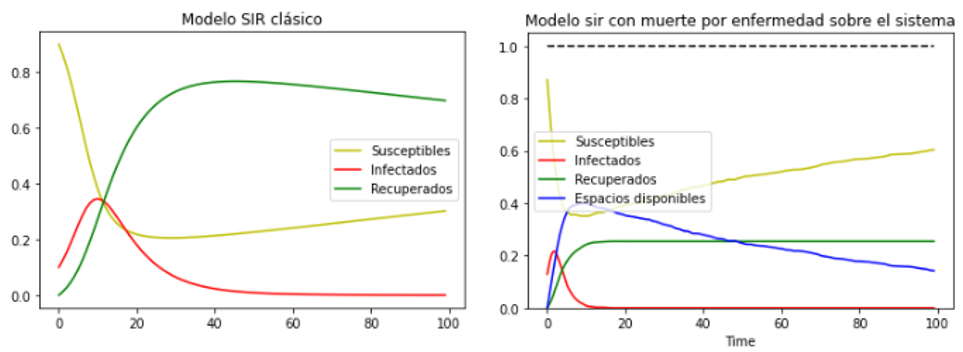
\includegraphics[width=0.95\textwidth]{Imagenes/solucionesMuertePorEnfermedad.PNG}
    \caption{Evolución de la enfermedad en 100 bimestres (modelo clásico y regla $\theta_{SIR,6}^t(x)$)}
    \label{fig:evolución100bimestres}
\end{figure}
En la figura (\ref{fig:evolución100bimestres}) se evidencia un pico para la enfermedad en las primeras iteraciones, esto debido principalmente a la alta tasa de contagio. Sin embargo, la alta tasa de muerte causada por la enfermedad hace que la población infectada desaparezca rápidamente como observa en ambos modelos.

Una diferencia significativa se puede apreciar en la cantidad de contagios. En el caso del modelo en autómatas celulares podemos afirmar que el número de contagios pudo no haber crecido en gran medida por algo como lo que se observa en la figura (\ref{fig:muertePorEnfermedad10Veces}), en donde las limitadas relaciones de las células hacen que los individuos infectados tiendan a aislarse.
\end{example}

En el siguiente capítulo abordaremos el caso de una enfermedad simulada sobre un espacio de células con relaciones específicas. Comenzando por la definición de los grados y tasas de impacto en el sistema y pasando por la aplicación de uno de los modelos epidemiológicos, podremos identificar algunas diferencias al usar un sistema u otro de vecindades.
